\section{Synchronisation}
\label{section:node-level:synchronisation}

Parallelisation schemes suffering from too much overhead are often subject of too much synchronisation.
Many threads might run in parallel, but if they permanently hit areas protected by semaphores (critical sections in OpenMP), i.e.~if they synchronise each other, the code cannot scale.
 

\begin{hypothesis}
 There are too many critical sections that cannot be entered by more than one thread, such that the threads tend to synchronise each other.
\end{hypothesis}


\noindent
Depending on the type of synchronisation, it will manifest in different behaviour that we can measure:
If locking mechanisms rely on spinning (busy waiting until a lock is released), we should see a high overhead in the underlying threading runtime.
If users implement locking themselves by try-locking over and over again until they get a resource, we either see a lot of these 
``try to lock'' calls, or we spend a lot of time in some kind of \texttt{yield} until a thread finally is successful in entering a critical section.


\paragraph{Data collection}

If our hypothesis holds, then we should see this (partial) synchronisation/serialisation in several metrics:

\begin{itemize}
  \item The effective CPU time (in the user code) is low compared to the actual execution time.
  \item There is a huge spin time.
  \item We see a massive lock contention.
\end{itemize}

\noindent

\begin{instructions}{\vtune}
In \vtune, too many synchronisation statements materialise in a high spin time as compared to the effective time.  
This leads to a low effective CPU utilisation (below is an example with eight cores, where we effectively only use four of them).
We also see that this synchronisation is caused by failed locks, which then make the scheduler yield. 

\begin{center}
 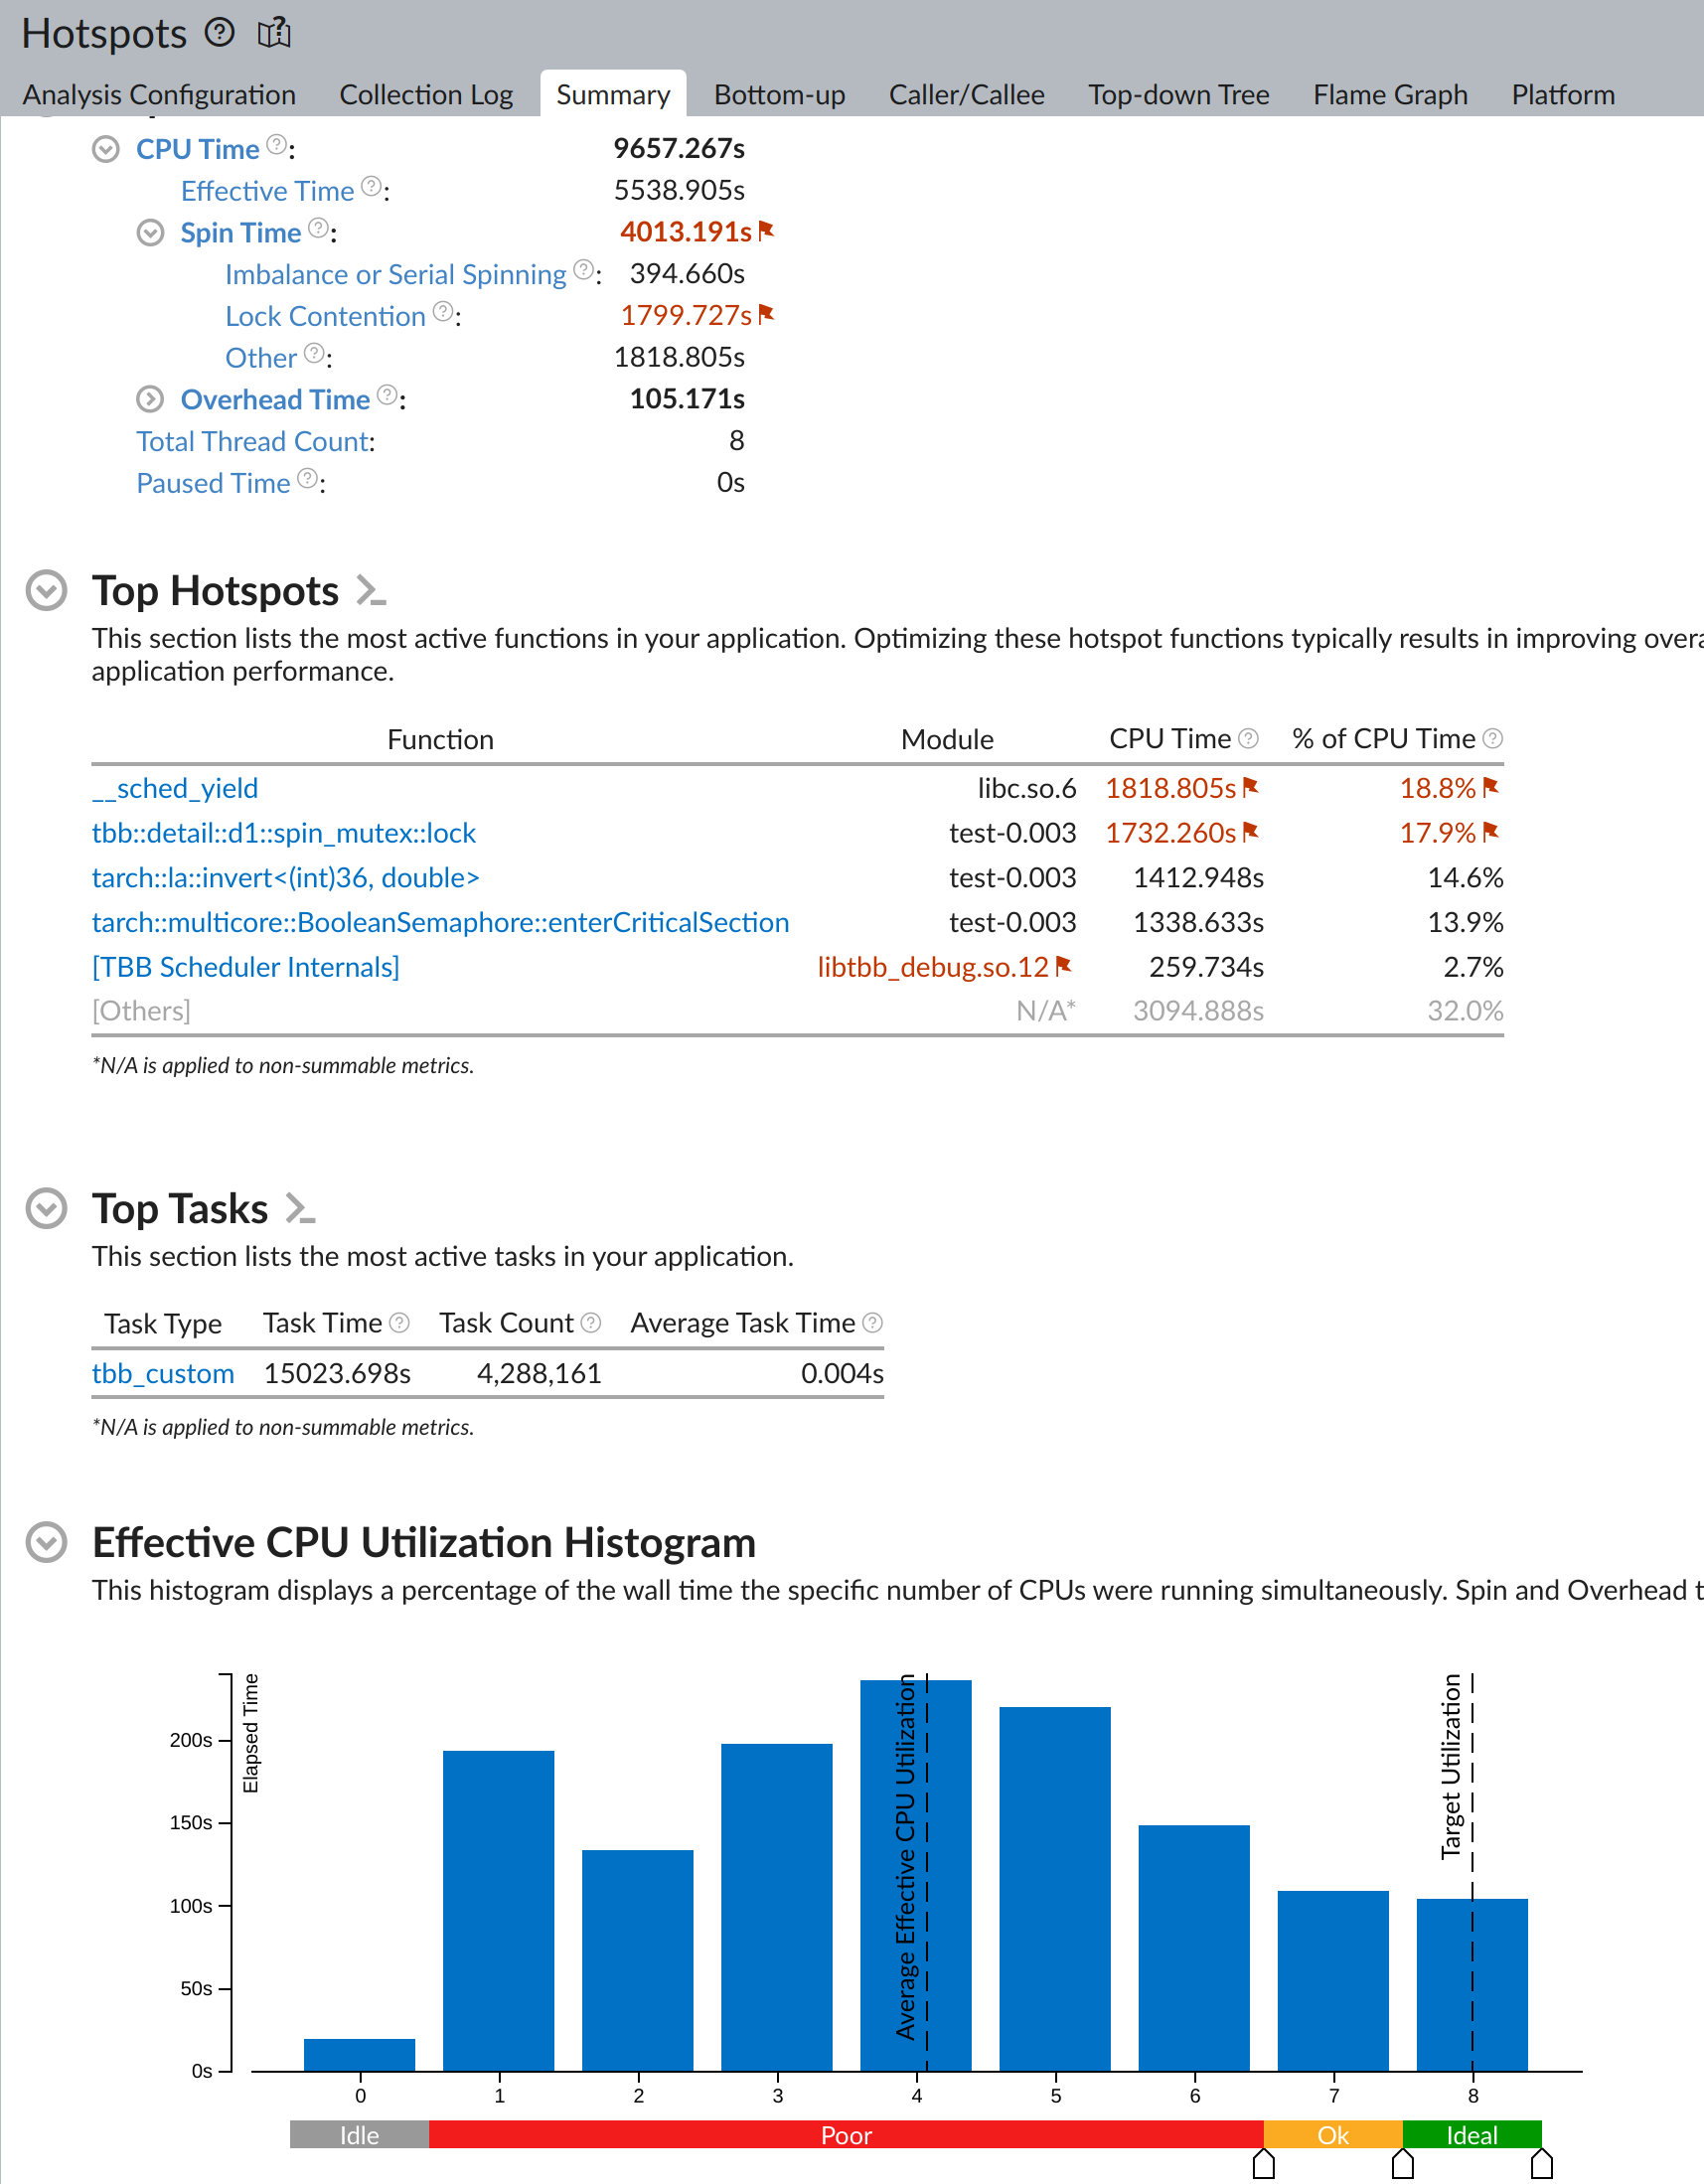
\includegraphics[width=0.5\textwidth]{node-level/synchronisation-vtune.png}
\end{center}

\noindent
With Intel Threading Building Blocks (TBB), we can switch to the \emph{Bottom-up} view and narrow down the relevant program phase (Section~\ref{section:tools:localisation}).
In the tabs, we might see significant amount of \emph{Lock Contention}.
\end{instructions}


\paragraph{Evaluation}

If the spin time or overhead time in the area of interest exceeds 20\% of the total execution time, i.e.~if the time we actually spend in our code underruns 80\% of the total time, we have a severe synchronisation flaw.


\paragraph{Optimisation and follow-up steps}

Remove
atomic variables



\paragraph*{How it works}

\begin{itemize}[noitemsep]
  \item[$\boxplus$] Validate that the administrative (non-science) fraction of the code scales with the scientific core calculations.
\end{itemize}


\paragraph*{How it does not work}

\begin{itemize}[noitemsep]
  \item[$\boxminus$] The administrative overhead will always increase relatively, so an increase in itself is not a flaw. An extraordinary increase coupled with limited scalability however is.
\end{itemize}
